Để kiểm thử tính sẵn sàng của hệ thống, nhóm sử dụng công cụ k6 – một công cụ mã nguồn mở cho phép mô phỏng nhiều người dùng đồng thời truy cập vào hệ thống.
\subsubsubsection{Cấu hình kiểm thử}
Kịch bản kiểm thử được thiết lập theo mô hình tăng tải tuần tự:

\begin{lstlisting}[frame=single, basicstyle=\small\ttfamily, breaklines=true, commentstyle=\color{gray}\itshape]
const options = {
     thresholds: {
        http_req_failed: ['rate<0.05'],
        http_req_duration: ['p(95)<2000'],  
    },
    scenarios: {
        api_test: {
            executor: 'ramping-vus',
            startVUs: 0,
            stages: [
                { duration: '30s', target: 50  },  // warm-up: 50 VU
                { duration: '1m',  target: 100 },  // tang dan toi 100 VU
                { duration: '30s', target: 0   },  // ha tai dan
            ],
            exec: 'runApiTest',
        },
    },
};
\end{lstlisting}
Trong đó:
\begin{itemize}
    \item \textbf{thresholds}: định nghĩa ngưỡng chấp nhận.
          \begin{itemize}
              \item \textbf{http\_req\_failed}: tỉ lệ yêu cầu thất bại. Với ngưỡng 0.05, k6 sẽ báo failure nếu có hơn 5\% yêu cầu lỗi.
              \item \textbf{http\_req\_duration}: thời gian phản hồi của các yêu cầu. Ngưỡng 2000ms (2 giây) đảm bảo trải nghiệm người dùng luôn mượt mà.
          \end{itemize}
    \item \textbf{stages}: định nghĩa số lượng người dùng ảo thay đổi theo thời gian.
          \begin{itemize}
              \item Giai đoạn đầu (30s, 50 VU) đóng vai trò warm-up để khởi động hệ thống.
              \item Giai đoạn hai (1m, 100 VU) mô phỏng tải cực đại.
              \item Giai đoạn cuối (30s, 0 VU) nhằm giải phóng tài nguyên, đảm bảo hạ tải an toàn.
          \end{itemize}
\end{itemize}

\subsubsubsection{Kết quả kiểm thử}
\begin{figure}[H]
    \centering
    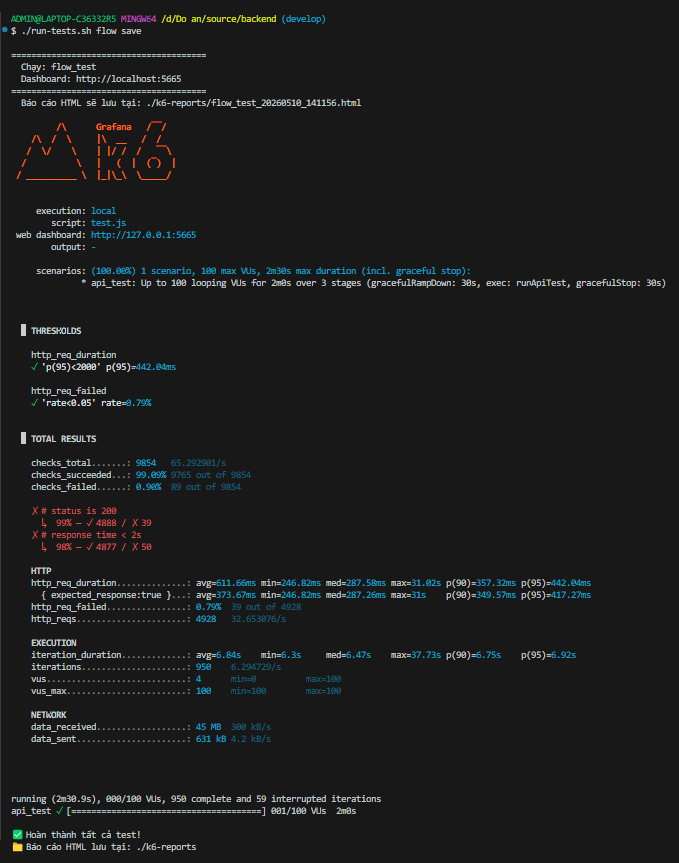
\includegraphics[width=\linewidth]{Images/8. Implement/backend/availability_evaluation.png}
    \caption{Kết quả kiểm thử tính sẵn sàng của hệ thống}
    \label{fig:availability-test}
\end{figure}
\subsubsubsection{Phân tích}
\begin{itemize}
    \item \textbf{Checks}: 99.09\% các yêu cầu vượt qua kiểm thử, còn lại 0.90\% thất bại (89 trường hợp).

    \item \textbf{Thời gian phản hồi trung bình}:
          \begin{itemize}
              \item[\textendash] Tất cả request: avg = \textbf{611.66ms}, p(90) = 357.32ms, p(95) = 442.04ms.
              \item[\textendash] Với các phản hồi hợp lệ (expected\_response = true): avg = \textbf{173.67ms}, trong đó 95\% request nằm trong khoảng $<$ \textbf{417.27ms}.
              \item[\textendash] Trung vị (\textit{median}) = 287.58ms, cho thấy đa số request thực tế phản hồi rất nhanh.
          \end{itemize}

    \item \textbf{Tỉ lệ lỗi}: 0.79\% request thất bại (39 trên 4928 request), chủ yếu do một số API phức tạp có response time vượt ngưỡng 2 giây.

    \item \textbf{Thông lượng}: hệ thống xử lý trung bình 32.65 request/giây với 100 người dùng ảo đồng thời (tổng 4928 requests).

    \item \textbf{Tài nguyên mạng}: dữ liệu nhận về đạt 45 MB (300 kb/s), dữ liệu gửi đi 631 kB (4.2 kb/s). Thời gian kết nối và thời gian chờ rất nhỏ (micro giây), chứng tỏ nghẽn chủ yếu nằm ở khâu xử lý trên server chứ không phải mạng.

    \item \textbf{Iteration duration}: trung bình 6.84s, với 95\% vòng lặp kết thúc dưới 6.92s. Một số request cá biệt chậm tới 37.73s, tuy nhiên không ảnh hưởng đáng kể đến p(95) do chiếm tỉ lệ rất nhỏ. Tổng số 950 vòng lặp hoàn thành với tốc độ 6.20 iterations/giây.
\end{itemize}

\subsubsubsection{Kết luận}
Kết quả kiểm thử cho thấy hệ thống đáp ứng tốt yêu cầu phi chức năng về tính sẵn sàng: cả hai ngưỡng kiểm thử đều đạt, tỉ lệ lỗi chỉ 0.79\% và thời gian phản hồi ở phân vị thứ 95 là 442ms – thấp hơn nhiều so với ngưỡng 2 giây. Phần lớn request hoàn thành dưới 300ms, đảm bảo trải nghiệm người dùng mượt mà khi có 100 người dùng đồng thời. Tuy nhiên, một số request ngoại lệ có thể kéo dài tới 31 giây, do đó cần tiếp tục tối ưu các API phức tạp và thao tác cơ sở dữ liệu ở phía backend để loại bỏ hoàn toàn các trường hợp chậm trễ này.